\section{Definicija derivacije}
\begin{definition}
Neka je $I\subseteq \mathbb{R}$ otvoreni interval. Kažemo da je $f : I\to \mathbb{R}$ \textbf{diferencijabilna} (ili \textit{derivabilna}) u točki $c\in I$ ako postoji $\lim\limits_{x\to c}{\dfrac{f(x)-f(c)}{x-c}}\in \mathbb{R}$. Taj broj zovemo \textbf{derivacija} funkcije $f$ u točki $c$ i označavamo ga s $f'(c)$. Nadalje, kažemo da je $f$ \textbf{diferencijabilna na $I$} ako je diferencijabilna u svakoj točki intervala $I$.
\end{definition}
Često se koristi i oznaka $\dfrac{\mathrm{d}f}{\mathrm{d}x}(c)$.

Ako je $I\subseteq \mathbb{R}$ otvoreni interval i $f : I\to \mathbb{R}$ diferencijabilna na $I$, onda funkciju $x\mapsto f'(x)$ zovemo \textbf{derivacija} funkcije $f$. Tako definiranu funkciju označavamo s $f'$, $\left(f(x)\right)'$, $\dfrac{\mathrm{d}f}{\mathrm{d}x}$, ili s $\dfrac{\mathrm{d}}{\mathrm{d}x}\left(f(x)\right)$.
\begin{remark}
Neka je $I\subseteq \mathbb{R}$ otvoreni interval. Tada je $f : I\to \mathbb{R}$ diferencijabilna u $c\in I$ ako i samo ako postoji $\lim\limits_{h\to 0}{\dfrac{f(c+h)-f(c)}{h}}$. Tada je
$$f'(c)=\lim\limits_{h\to 0}{\dfrac{f(c+h)-f(c)}{h}}.$$
\end{remark}
\begin{definition} Neka je $I\subseteq \mathbb{R}$ otvoreni interval i $c\in I$. Ako postoji limes $\lim\limits_ {x\to c+}{\dfrac{f(x)-f(c)}{x-c}}\in \mathbb{R}$, taj broj zovemo \textbf{desna derivacija} funkcije $f$ u točki $c$ i označavamo ga s $f_d'(c)$. Analogno, ako postoji limes $\lim\limits_ {x\to c-}{\dfrac{f(x)-f(c)}{x-c}}\in \mathbb{R}$, zovemo ga \textbf{lijeva derivacija} funkcije $f$ u točki $c$ i označavamo ga s $f_l'(c)$.
\end{definition}
\begin{exercise} \textbf{}
\label{firstder}
\begin{itemize}
\item[a)] Dokažite da je $x\mapsto x^3$ diferencijabilna na $\mathbb{R}$ i odredite joj derivaciju.
\item[b)] Je li $f : \mathbb{R}\to \mathbb{R}$,
$$f(x)=\begin{cases}
x^3, & x\geq 0,\\
x, & x\leq 0.
\end{cases}$$
diferencijabilna na $\mathbb{R}$?
\end{itemize}
\end{exercise}
\begin{proof}[Rješenje]
a) Neka je $c\in \mathbb{R}$ proizvoljan. Vrijedi
$$\lim\limits_{x\to c}{\dfrac{x^3-c^3}{x-c}}=\lim\limits_{x\to c}{\dfrac{(x-c)(x^2+xc+c^2)}{x-c}}=\lim\limits_{x\to c}{\left(x^2+xc+c^2\right)}=3c^2.$$
Dakle, za sve $c\in \mathbb{R}$, $x\mapsto x^3$ je diferencijabilna u $c$ i vrijedi $f'(c)=3c^2$. Stoga je derivacija funkcije $x\mapsto x^3$ funkcija $x\mapsto 3x^2$.

b) Tvrdimo da $f$ nije diferencijabilna u $0$. Zaista, vrijedi $$f_d'(0)=\lim\limits_{x\to 0+}{f'(x)}=\lim\limits_{x\to 0+}{\dfrac{x^3}{x}}=0,$$
a s druge strane imamo 
$$f_l'(0)=\lim\limits_{x\to 0-}{f'(x)}=\lim\limits_{x\to 0-}{\dfrac{x}{x}}=1,$$
dakle $f$ nije diferencijabilna na $\mathbb{R}$.
\end{proof}

\begin{exercise} \textbf{}
\begin{itemize}
\item[a)] Navedite primjer funkcije $f : \mathbb{R}\to \mathbb{R}$ takve da je $f'(1)=1$ i $f'(5)=2$.
\item[b)] Navedite primjer funkcije $f : \mathbb{R}\to \mathbb{R}$ koja je neprekidna na $\mathbb{R}$, te diferencijabilna svugdje osim u točkama $1$ i $2$.
\end{itemize}
\end{exercise}
\begin{proof*}
a) Znamo da je npr. za $a\in \mathbb{R}$, $\left(ax\right)'=a$, stoga možemo uzeti npr. $f : \mathbb{R}\to \mathbb{R}$,
$$f(x)=\begin{cases}
x, & x\leq 2,\\
5x, & x\geq 2.
\end{cases}$$
Primijetimo da je $f'(1)=1$. Zaista, očito vrijedi
\[
\pushQED{\qed}
\lim\limits_{x\to 1}{\dfrac{f(x)-f(1)}{x-1}}=\lim\limits_{x\to 1}{\dfrac{x-1}{x-1}}=1.\qedhere
\popQED
\]
\end{proof*}
\begin{remark}
Neka je $I\subseteq \mathbb{R}$ otvoreni interval i $f : I \to \mathbb{R}$ diferencijabilna u točki $c\in I$. Tada je $f$ i neprekidna u $c$.
\end{remark}
Obrat gornje napomene općenito ne vrijedi, i to npr. za funkciju $x\mapsto |x|$. Intuitivno, klasični primjeri funkcija koje su neprekidne ali ne i diferencijabilne u nekoj točki su one čiji grafovi imaju "šiljak" u toj točki.
\begin{exercise} \textbf{}
\label{idkhowtonamethis}
\begin{itemize}
\item[a)] Postoji li $c>0$ takav da je $f : \mathbb{R}\to \mathbb{R}$,
$$f(x)=\begin{cases}
cx^3,& x\geq 0,\\
-x^2-1-c,& x<0.
\end{cases}$$
diferencijabilna na $\mathbb{R}$?
\item[b)] Odredite sve $a, b\in \mathbb{R}$ takve da je $g : \mathbb{R}\to \mathbb{R}$,
$$g(x)=\begin{cases}
x^3,& x\leq 1,\\
ax+b,& x>1.
\end{cases}$$
diferencijabilna na $\mathbb{R}$.
\item[c)] Odredite neku funkciju $F : \langle -3, 3\rangle\to \mathbb{R}$ takvu da funkcija $c:\mathbb{R}\to \mathbb{R}$,
$$c(x)=\begin{cases}
-8,& x\leq -3,\\
F(x),& x\in \langle -3, 3\rangle,\\
8,& x\geq 3.
\end{cases}$$
bude diferencijabilna na $\mathbb{R}$.
\end{itemize}
\end{exercise}
\begin{proof}[Rješenje]
a) Pretpostavimo da postoji takav $c>0$. Da bi $f$ bila diferencijabilna u $0$, mora biti i neprekidna u $0$. Vrijedi
$$\lim\limits_{x\to 0+}{f(x)}=\lim\limits_{x\to 0+}{cx^3}=0,\;\; \lim\limits_{x\to 0-}{f(x)}=\lim\limits_{x\to 0-}{-x^2-1-c}=-1-c,$$
Kako je $-1-c<0$, lijevi i desni limes ne mogu biti jednaki, pa ne postoji takav $c$.

b) Slično kao i u a), uspoređivanjem lijevog i desnog limesa vidimo da mora vrijediti $a+b=1$. S druge strane, imamo $g_d'(1)=a$ i analogno $g_l'(1)=3$, stoga mora vrijediti $a=3$. Odavde imamo da je $b=-2$. Očito je za ovako odabrane $a$ i $b$ funkcija $g$ diferencijabilna u $1$. Ako je $x>1$, onda je $g'(x)=\dfrac{\mathrm{d}}{\mathrm{d}x}(ax+b)=a$, a za $x<1$ imamo $g'(x)=\dfrac{\mathrm{d}}{\mathrm{d}x}(x^3)=3x^2$. Stoga je $g$ diferencijabilna na $\mathbb{R}$ ako i samo ako je $a=3$ i $b=-2$.

c) Funkcija $f : \mathbb{R}\to \mathbb{R}$, $f(x)=x^3$ ima svojstvo $f'(0)=0$, pa će ideja biti njezin graf translatirati tako da točka ishodišta prijeđe u npr. točku $(-3, 8)$, tj. za $3$ jedinične dužine ulijevo i $8$ jediničnih dužina prema dolje (te ga, naravno, i restringirati tako da konačna funkcija $F$ ima domenu $\langle -3, 3\rangle$). Tražena funkcija je (v. napomenu \ref{graphrem}) $g : \langle -3, 1]\to \mathbb{R}$, 
$$g(x)=(x+3)^3-8,$$
(v. sliku \ref{dergraph}). Uočimo da je $g$ "na pola puta" između $-8$ i $8$ gledajući po $y$-osi upravo u svojoj nultočki, tj. točki $(-1,0)$, pa će sada biti ideja uzeti funkciju $h : [-1, 1]\to \mathbb{R}$ koja će biti pogodna translacija dijela "lijevog dijela" grafa funkcije $x\mapsto (x+3)^3-8$, tako da iz točke $(-1, 0)$ dođemo do točke $(1, 8)$, na način da vrijedi $h_d'(1)=0$. Uočimo da je $g'(-1)=12$, te je broj $a\in \mathbb{R}$, $a\neq -1$ takav da je $g'(a)=12$, broj $a=-5$, pa kako želimo da se desna derivacija od $g$ te lijeva derivacija od $h$ u točki $-1$ i njihove funkcijske vrijednosti u toj točki podudaraju, zahtijevati ćemo da točka $(-5, -16)$ prijeđe u točku $(-1, 0)$. Slijedi da graf funkcije $g$ moramo translatirati za $4$ jedinične dužine udesno i $16$ jediničnih dužina prema gore, čime dobivamo 
$$h(x)=(x-1)^3+8.$$ Sada je $h(1)=8$ i $h_d'(1)=0$, pa kako bi došli do točke $(3, 8)$ možemo iskoristiti dio grafa konstantne funkcije $x\mapsto 8$. Dakle, tražena funkcija biti će $F : \langle -3, 3\rangle\to \mathbb{R}$,
$$F(x)=\begin{cases}
(x+3)^3-8, & x\in \langle -3, -1],\\
(x-1)^3+8, & x\in [-1, 1],\\
8, & x\in [1, 3\rangle.
\end{cases}$$
Nije teško provjeriti da je $F$ zaista diferencijabilna na $\mathbb{R}$.
\begin{figure}[ht]
\begin{subfigure}[t]{.5\textwidth}
\centering
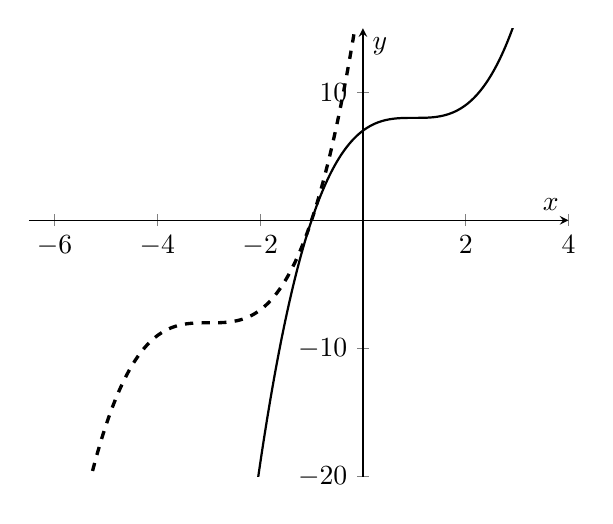
\begin{tikzpicture}
\begin{axis}[axis lines=middle,xlabel=$x$,ylabel=$y$,xmin=-6.5,xmax=4,ymin=-20,ymax=15, smooth, samples=200]

\addplot[very thick,dashed,color=black,domain=-8:1] {(x+3)^3-8};
\addplot[thick,color=black,domain=-3:3] {(x-1)^3+8};
\end{axis}
\end{tikzpicture}
\caption*{Grafovi funkcija $x\mapsto (x+3)^3-8$ (iscrtkana linija) i $x\mapsto (x-1)^3+8$ (puna linija)}
\end{subfigure}%
\begin{subfigure}[t]{.5\textwidth}
\centering
\begin{tikzpicture}
\begin{axis}[axis lines=middle,xlabel=$x$,ylabel=$y$,xmin=-6.5,xmax=4,ymin=-20,ymax=15, smooth, samples=200]

\addplot[thick,dotted,color=black,domain=-20:-3] {-8};
\addplot[very thick,dashed,color=black,domain=-3:-1] {(x+3)^3-8};
\addplot[thick,color=black,domain=-1:1] {(x-1)^3+8};
\addplot[very thick,dashdotted,color=black,domain=1:3] {8};
\addplot[thick,dotted,color=black,domain=3:4] {8};
\end{axis}
\end{tikzpicture}
\caption*{Graf funkcije $F$ iz rješenja c) dijela zadatka \ref{idkhowtonamethis}}
\end{subfigure}
\caption{\label{dergraph}}
\end{figure}
\end{proof}
\newpage
\begin{exercise} 
\label{localder}
Neka je $I\subseteq \mathbb{R}$ otvoreni interval i $f : I \to \mathbb{R}$ diferencijabilna u $c\in I$. Dokažite da ako je $f'(c)>0$, da tada postoji $\delta>0$ takav da vrijedi
$$
\begin{cases}
x\in \langle c-\delta, c\rangle\cap I\Rightarrow f(x)<f(c),\\
x\in \langle c, c+\delta\rangle\cap I\Rightarrow f(x)>f(c).
\end{cases}
$$
\end{exercise}
\begin{proof}[Rješenje]
Po definiciji, za $\epsilon=f'(c)$ postoji $\delta>0$ takav da za sve $x\in I$ takve da je $0<|x-c|<\delta$ vrijedi
$$0<\dfrac{f(x)-f(c)}{x-c}<2f'(c)$$
Ako je $x>c$, tj. $x\in \langle c,c+\delta\rangle\cap I$, tada množenjem nejednakosti $0<\dfrac{f(x)-f(c)}{x-c}$ s $x-c$ dobivamo $f(x)>f(c)$. Analogno za $x<c$, odnosno $x\in \langle c-\delta, c\rangle\cap I$ dobivamo $f(x)<f(c)$.
\end{proof}

\begin{exercise}
Dokažite da je $x\mapsto \ln{x}$ diferencijabilna na $\langle 0,\infty\rangle$ i odredite joj derivaciju.
\end{exercise}
\begin{proof}[Rješenje]
Neka je $c>0$ proizvoljan. Imamo
$$\lim\limits_{x\to c}{\dfrac{\ln{x}-\ln{c}}{x-c}}=\lim\limits_{x\to c}{\dfrac{\ln{\dfrac{x}{c}}}{x-c}}=\lim\limits_{x\to c}{\ln\left(\left(\dfrac{x}{c}\right)^\frac{1}{x-c}\right)}.$$
Uočimo da vrijedi
$$\lim\limits_{x\to c}{\left(\dfrac{x}{c}\right)^\frac{1}{x-c}}=\lim\limits_{x\to c}{\left(\dfrac{x-c+c}{c}\right)^\frac{1}{x-c}}=\lim\limits_{x\to c}{\left(1+\dfrac{x-c}{c}\right)^\frac{1}{x-c}}=\lim\limits_{x\to c}{\left(\left(1+\dfrac{x-c}{c}\right)^\frac{c}{x-c}\right)^\frac{1}{c}}.$$
Želimo supstituirati $y=\dfrac{x-c}{c}$, pa se želimo uvjeriti da su zadovoljeni svi uvjeti teorema 13 u \cite{14}. Zaista, neka su $f, g : \langle 0, \infty\rangle\setminus\{c\}\to \mathbb{R}$ dane s 
$$f(x)=\left((1+x)^\frac{1}{x}\right)^\frac{1}{c},\;\;\;\;g(x)=\dfrac{x-c}{c}.$$ 
Tada je $f\circ g$ definirana na $\langle 0, \infty\rangle\setminus\{c\}$, $f$ ima limes $0$ u $c$ i $g$ ima limes u $e^\frac{1}{c}$ u $0$, te npr. za $\epsilon=c$ vrijedi da je $f(x)\neq 0$ za sve $x\in \langle c-\epsilon, c+\epsilon\rangle$, $x\neq c$, budući da je na tom intervalu $f$ strogo monotona. Stoga je
$$\lim\limits_{x\to c}{\left(\dfrac{x}{c}\right)^\frac{1}{x-c}}=\lim\limits_{x\to c}{\left(\left(1+\dfrac{x-c}{c}\right)^\frac{c}{x-c}\right)^\frac{1}{c}}=\lim\limits_{y\to 0}{\left((1+y)^\frac{1}{y}\right)^\frac{1}{c}}=e^\frac{1}{c}.$$
Odavde i iz činjenice da je $\ln$ neprekidna u $c$ $\left(\text{pa ima limes u }f(c)\right)$ i strogo rastuća, analognom primjenom teorema 13 u \cite{14} slijedi
$$\lim\limits_{x\to c}{\ln\left(\left(\dfrac{x}{c}\right)^\frac{1}{x-c}\right)}=\ln{e^\frac{1}{c}}=\dfrac{1}{c}.$$
Stoga je $\ln$ diferencijabilna na $\langle 0, \infty\rangle$ i njezina derivacija je $x\mapsto \dfrac{1}{x}$.
\end{proof}
\begin{exercise}
Neka je $I\subseteq \mathbb{R}$ otvoreni interval i $f : I \to \mathbb{R}$ diferencijabilna na $I$. Koristeći do sada poznate rezultate, dokažite da ako za sve $x\in I$ vrijedi $f'(x)\geq 0$, da je tada $f$ rastuća.
\end{exercise}
\begin{proof}[Rješenje]
Pretpostavimo suprotno, tj. da postoje $x_1, x_2\in I$ takvi da je $x_1<x_2$, ali $f(x_1)>f(x_2)$. Ideja dokaza će biti sljedeća -- u segmentu $[x_1, x_2]$ ćemo promotriti najveći element za koji $f$ postiže maksimum na tom segmentu. Najprije ćemo dokazati da taj najveći element uopće postoji i to tako da ga definiramo kao supremum svih elemenata koji postižu maksimum na segmentu. Svaki element u segmentu strogo veći od tog elementa će dakle biti strogo manji od tog elementa, što će biti u kontradikciji sa zadatkom \ref{localder}.

Neka je 
$$S=\left\{x\in [x_1, x_2] : f(x)=\max{f|_{[x_1, x_2]}}\right\}.$$ 
Uočimo da je $f$ neprekidna na segmentu $[x_1, x_2]$ i na tom segmentu nije konstanta, pa postoji bar jedan $x_i\in [x_1, x_2]$ takav da je $f(x_i)=\max{f|_{[x_1, x_2]}}$. Dakle, postoji $\sup{S}$.

Tvrdimo da je $\sup{S}\neq x_2$. Zaista, po zadatku \ref{localder} postoji $\delta>0$ takav da za sve $x\in \langle x_2-\delta, x_2\rangle\cap I$ vrijedi $f(x)<f(x_2)$. S druge strane, po lemi \ref{14} imamo da za $\epsilon=\delta$ postoji $x_0\in [x_1, x_2]$ takav da je $f(x_0)=\max{f|_{[x_1, x_2]}}$ i vrijedi $x_2-\delta<x_0$. Pritom vrijedi $x_0<x_2$, jer kad bi bilo $x_0=x_2$, onda bi vrijedilo $f(x_2)=\max{f|_{[x_1, x_2]}}$, što je kontradikcija s činjenicom da je $f(x_2)<f(x_1)$. Sada iz činjenice da je $x_0\in \langle x_2-\delta, x_2\rangle\cap I$ slijedi da je $f(x_0)<f(x_2)$, što je kontradikcija s činjenicom da je $f(x_0)=\max{f|_{[x_1, x_2]}}$.

Kako je $S\subseteq [x_1, x_2]$, to je $\sup{S}\leq \sup{[x_1, x_2]}=x_2$, pa iz činjenice da je $\sup{S}\neq x_2$ imamo da je $\sup{S}<x_2$. Dokažimo i da je
$\sup{S}=\max{S}.$
Zaista, po lemi \ref{14} za svaki $n\in \mathbb{N}$ postoji $z_n\in [x_1, x_2]$ takav da je $f(z_n)=\max{f|_{[x_1, x_2]}}$ i vrijedi $\sup{S}-\dfrac{1}{n}<z_n$. Promotrimo niz $(z_n)$. Očito vrijedi $z_n\leq \sup{S}$, pa po kriteriju sendviča imamo $\lim\limits_{x\to\infty}{z_n}=\sup{S}$, pa iz činjenice da je $f$ diferencijabilna, pa i neprekidna u $\sup{S}$ slijedi
$$f(\sup{S})=\lim\limits_{x\to\infty}{f(z_n)}=\lim\limits_{x\to\infty}{\max{f|_{[x_1, x_2]}}}=\max{f|_{[x_1, x_2]}}.$$
Odavde imamo da je $\sup{S}\in S$, pa je i $\sup{S}=\max{S}$.

Konačno, kako je $f'(\max{S})>0$, postoji $\delta>0$ takav da za sve $x\in \langle \max{S}, \max{S}+\delta\rangle\cap I$ vrijedi $f(x)>f(\max{S})$. Neka je $\delta'=\min\{\delta, x_2-\max{S}\}$. Tada je 
$$\max{S}+\delta'\leq \max{S}+x_2-\max{S}=x_2,$$
pa za sve $\langle \max{S}, \max{S}+\delta'\rangle\cap I\subseteq \langle \max{S}, x_2\rangle$ vrijedi $f(x)>f(\max{S})$. No ovo znači da npr. vrijedi $$f\left(\max{S}+\dfrac{\delta'}{2}\right)>f(\max{S}).$$ S druge strane, kako je $\max{S}+\dfrac{\delta'}{2}\in [x_1, x_2]$ i $\max{S}+\dfrac{\delta'}{2}>\max{S}$, vrijedi $\max{S}+\dfrac{\delta'}{2}\notin S$,
pa je $f\left(\max{S}+\dfrac{\delta'}{2}\right)<\max{f|_{[x_1, x_2]}}=f(\max{S})$, kontradikcija!
\end{proof}
\section{Osnovne operacije s diferencijabilnim funkcijama}
\begin{remark}[Osnovne operacije s diferencijabilnim funkcijama]
Neka je $I\subseteq \mathbb{R}$ otvoreni interval, te $f, g : I\to \mathbb{R}$ diferencijabilne u točki $c\in I$. Tada vrijede sljedeće tvrdnje.
\begin{itemize}
\item[a)] Funkcija $f+g$ je diferencijabilna u $c$ i vrijedi $(f+g)'(c)=f'(c)+g'(c)$,
\item[b)] Funkcija $fg$ je diferencijabilna u $c$ i vrijedi $(fg)'(c)=f'(c)g(c)+f(c)g'(c)$,
\item[c)] Ako je $g(c)\neq 0$, onda je $\left(\dfrac{f}{g}\right)$ diferencijabilna u $c$ i vrijedi $$\left(\dfrac{f}{g}\right)'(c)=\dfrac{f'(c)g(c)-f(c)g'(c)}{g(c)^2}.$$ 
\end{itemize}
\end{remark}
\begin{remark}[Derivacije elementarnih funkcija] Sljedeće tvrdnje vrijede za sve $x$ iz prirodne domene pripadnih funkcija.
\begin{AutoMultiColItemize}
\item $(c)'=0$, gdje je $c\in \mathbb{R}$
\item $(x^a)'=ax^{a-1}$, gdje je $a\in\mathbb{R}$,
\item $(\sin{x})'=\cos{x}$,
\item $(\cos{x})'=-\sin{x}$,
\item $(\tg{x})'=\dfrac{1}{\cos^2{x}}$,
\item $(\ctg{x})'=-\dfrac{1}{\sin^2{x}}$,
\item $(a^x)'=a^x\ln{a}$, gdje je $a>0$
\item $(e^x)'=e^x$,
\item $(\arcsin{x})'=\dfrac{1}{\sqrt{1-x^2}}$,
\item $(\arccos{x})'=-\dfrac{1}{\sqrt{1-x^2}}$,
\item $(\arctg{x})'=\dfrac{1}{1+x^2}$,
\item $(\arcctg{x})'=-\dfrac{1}{1+x^2}$,
\item $(\log_a{x})'=\dfrac{1}{x\ln{a}}$, gdje je $a>0, a\neq 1$,
\item $(\ln{x})'=\dfrac{1}{x}$,
\item $(\sh{x})'=\ch{x}$,
\item $(\ch{x})'=\sh{x}$,
\item $(\th{x})'=\dfrac{1}{\ch^2{x}}$,
\item $(\cth{x})'=-\dfrac{1}{\sh^2{x}}$
\end{AutoMultiColItemize}
\end{remark}